\documentclass[12pt]{article}
%%%%%%%%%%%%%%%%%%%%%%%%%%%%%%%%%%%%%%%%%%%%%%%%%%%%%
%%%%%%%%%%%  MATH  %%%%%%%%%%%%%%%%%%%%%%%%%%%%%%%%%%
\usepackage{amsmath,amsthm,amssymb} %math
\usepackage{xfrac} %sfrac
\usepackage{faktor} %better than sfrac
\usepackage{dutchcal} %some font for mathcal
\usepackage{array} %for newcoltype
\newlength\mylen
\newcolumntype{R}{>{\hfill$}p{\mylen}<{$}}
\settowidth\mylen{$-1$}
%\everymath{\displaystyle} %to show every math big
%%%%%%%%%%%%%%%%%%%%%%%%%%%%%%%%%%%%%%%%%%%%%%%%%%%%%
%%%%%%%%%%%  OTHER PACKAGES  %%%%%%%%%%%%%%%%%%%%%%%%
\usepackage[utf8]{inputenc} %encoding
\usepackage{hyperref} %hyperlinks
\usepackage{geometry} %page size and margins
\usepackage{makeidx} %indexing
\usepackage{graphicx} %inclusion of graphics
\usepackage{wrapfig} %wrap text around figures
\usepackage{xstring} %manipulate strings
\usepackage[dvipsnames]{xcolor} %colors !conflicts with beamer!
%%%%%%%%%%%%%%%%%%%%%%%%%%%%%%%%%%%%%%%%%%%%%%%%%%%%%
%%%%%%%%%%%  TIKZ 4 LIFE  %%%%%%%%%%%%%%%%%%%%%%%%%%%
\usepackage{tikz}
\usetikzlibrary{cd} %commutative diagrams
\usetikzlibrary{decorations} %curved lines
\usetikzlibrary{positioning} %coordinates positioning
%\usetikzlibrary{replacements} %right=of nodename
\usetikzlibrary{3d,calc} %coordinate calculations & 3d
%%%%%%%%%%%%%%%%%%%%%%%%%%%%%%%%%%%%%%%%%%%%%%%%%%%%%
%%%%%%%%%%%  CUSTOMIZE THE LOOKS  %%%%%%%%%%%%%%%%%%%
\geometry{headheight=15pt}
\setlength\parindent{0pt} %no indentation
%%%%%%%%%%%%%%%%%%%%%%%%%%%%%%%%%%%%%%%%%%%%%%%%%%%%%
%%%%%%%%%%%  ENUMERATE / ITEMIZE  %%%%%%%%%%%%%%%%%%%
\usepackage{enumerate} %enumerate/itemize (has to be first)
\usepackage{enumitem} %customize enumerate/itemize
 \setlist{nolistsep} %<=> [nosep] <=> Kills vert sep <=> ![listsep]
\newenvironment{n_enum}{\begin{enumerate}[label=(\arabic{*})]}{\end{enumerate}} %1,2,3,...
\newenvironment{i_enum}{\begin{enumerate}[label=(\roman{*})]}{\end{enumerate}} %i,ii,iii,...
\newenvironment{a_enum}{\begin{enumerate}[label=(\alph{*})]}{\end{enumerate}} %a,b,c,...
\newenvironment{b_item}{\begin{itemize}}{\end{itemize}} %bullets
%%%%%%%%%%%%%%%%%%%%%%%%%%%%%%%%%%%%%%%%%%%%%%%%%%%%%
%%%%%%%%%%%  MATH NOTATIONS  %%%%%%%%%%%%%%%%%%%%%%%%
\newenvironment{eqarray}{\begin{array}{>{\displaystyle}r>{\displaystyle}c>{\displaystyle}l}}{\end{array}}
\newcommand\Hom{\mathrm{Hom}}
\newcommand\NHom{\mathrm{NHom}}
\newcommand\ChRmod{Ch($R$-mod)}
\newcommand\ChZmod{Ch($\mathbb{Z}$-mod)}
\newcommand\KRmod{$\mathcal{K}$($R$-mod)}
\newcommand\Csing[1]{C^{\mathrm{sing}}\left(#1\right)}
\newcommand\Dtop[1]{\Delta^{\mathrm{top}}\left(#1\right)}
\newcommand\Tor{\mathrm{Tor}}
\newcommand\Ext{\mathrm{Ext}}
\newcommand\Mod{\mathrm{Mod}}
\newcommand\Ab{\mathrm{Ab}}
\newcommand\map{\mathrm{map }}
\newcommand\im{\mathrm{im\ }}
\newcommand\tensor{\otimes}
%\newcommand\ker{\mathrm{ker}}
\newcommand\coim{\mathrm{coim\ }}
\newcommand\coker{\mathrm{coker\ }}
\newcommand\cupdot{\mathbin{\mathaccent\cdot\cup}}
\newcommand\rank{\mathrm{rank}}
\newcommand\val{\mathrm{val}}
%%%%%%%%%%%%%%%%%%%%%%%%%%%%%%%%%%%%%%%%%%%%%%%%%%%%%
%%%%%%%%%%%  OTHER NOTATIONS  %%%%%%%%%%%%%%%%%%%%%%%
\newcommand\ul[1]{\emph{#1}}
\newcommand\nospace{\hspace*{-0.5em}}
\newcommand\HRule{\rule{\linewidth}{0.1mm}}
%%%%%%%%%%%%%%%%%%%%%%%%%%%%%%%%%%%%%%%%%%%%%%%%%%%%%
%%%%%%%%%%%  BEGIN DOCUMENT  %%%%%%%%%%%%%%%%%%%%%%%%
\begin{document}
\begin{center}
{\bf Mathematical Aspects of Public Transportation Networks}\\
Problem Set 9
\end{center}
So 2018 \hfill Dimitrios Bogiokas - BMS\\
\phantom{X}\hfill FU ID: 5048996\\
\HRule\\
{\bf Exercise 1} \begin{a_enum} \item A minimum cost circulation covering each driving activity includes (except for every driving activity) a perfect matching on every station. In K\"openick the perfect matching trivially contains the only transfer activity. In Lichtenberg and in Faltenberg there are two perfect matchings in each to choose from and one can easily find the ones that are of minimum cost. With a little help of a C++ program, which is included, one can see that in Sch\"oneweide every minimum weight matching has weight $37$. Thus we have with respect to $x$:
$$\begin{array}{rcl}\min
&=&(4\cdot44+2\cdot34+50+51+2\cdot24)+12+(10+8)+(10+10)+37\\
&=&393+12+18+20+37=480\\
\end{array}$$
\item Using the same program, we also get all particular matchings achieving cost $37$ in Sch\"oneweide. Thus one minimum-weight perfect matching of $(V,E_t)$ is:
\begin{center}
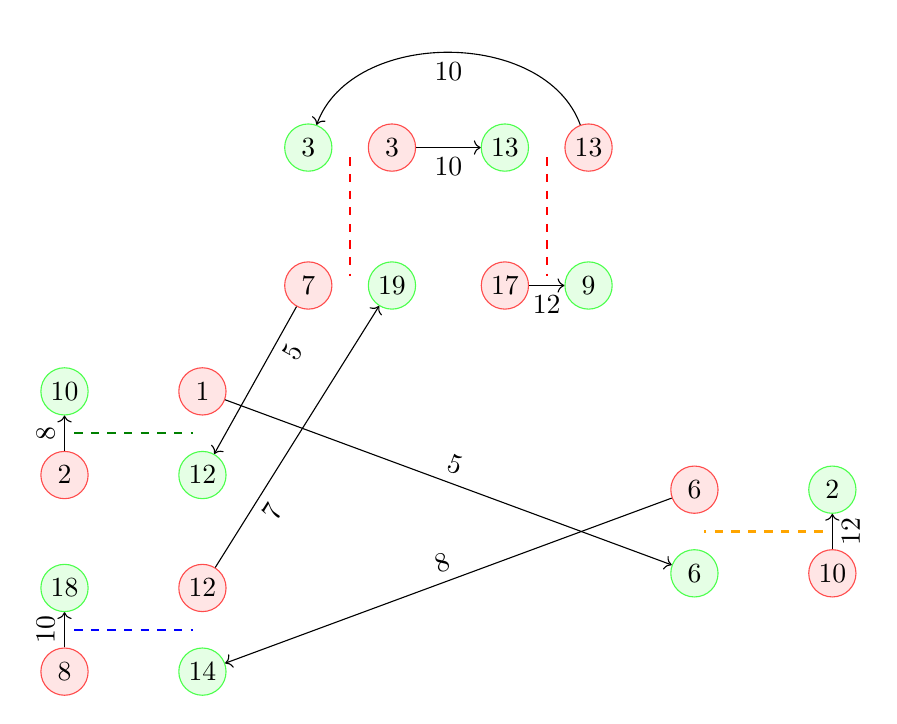
\begin{tikzpicture}[node distance = 3cm,
event/.style={circle, draw, minimum size = 6mm, inner sep = 0pt, node distance = .1cm},
eventd/.style={draw=green!70, fill=green!10, event},
eventa/.style={draw=red!70, fill=red!10, event},
line/.style={node distance = 1cm}]
\def\dist{8}
\def\a{above}
\def\b{below}
\def\l{left}
\def\r{right}
\def\al{above left}
\def\bl{below left}
\def\ar{above right}
\def\br{below right}
\coordinate (L) at (-\dist,0);
\coordinate (S) at (0,0);
\coordinate (K) at (\dist,0);
\coordinate (F) at (0,\dist);

\node (Lr) [\r=of L] {};
\node[line] (Lgr) [\a=of Lr] {};
\node[line] (Lbl) [\b=of Lr] {};
\node[eventd] (LgrD) [\a=of Lgr] {$10$};
\node[eventa] (LgrA) [\b=of Lgr] {$2$};
\node[eventd] (LblD) [\a=of Lbl] {$18$};
\node[eventa] (LblA) [\b=of Lbl] {$8$};

\node (Fb) [\b=of F] {};
\node[line] (Fr1) [\l=of Fb] {};
\node[line] (Fr2) [\r=of Fb] {};
\node[eventd] (Fr1D) [\l=of Fr1] {$3$};
\node[eventa] (Fr1A) [\r=of Fr1] {$3$};
\node[eventd] (Fr2D) [\l=of Fr2] {$13$};
\node[eventa] (Fr2A) [\r=of Fr2] {$13$};

\node (Kye) [\l=of K] [line] {};
\node[eventd] (KyeD) [\a=of Kye] {$2$};
\node[eventa] (KyeA) [\b=of Kye] {$10$};

\node (Sl) [\l=of S] {};
\node[line] (Sgr) [\a=of Sl] {};
\node[line] (Sbl) [\b=of Sl] {};
\node[eventd] (SgrD) [\b=of Sgr] {$12$};
\node[eventa] (SgrA) [\a=of Sgr] {$1$};
\node[eventd] (SblD) [\b=of Sbl] {$14$};
\node[eventa] (SblA) [\a=of Sbl] {$12$};

\node (Sa) [\a=of S] {};
\node[line] (Sr1) [\l=of Sa] {};
\node[line] (Sr2) [\r=of Sa] {};
\node[eventd] (Sr1D) [\r=of Sr1] {$19$};
\node[eventa] (Sr1A) [\l=of Sr1] {$7$};
\node[eventd] (Sr2D) [\r=of Sr2] {$9$};
\node[eventa] (Sr2A) [\l=of Sr2] {$17$};

\node (Sye) [\r=of S] [line] {};
\node[eventd] (SyeD) [\b=of Sye] {$6$};
\node[eventa] (SyeA) [\a=of Sye] {$6$};

\draw[->] (LblA) to node[above, sloped, swap] {$10$} (LblD);
\draw[->] (LgrA) to node[above, sloped, swap] {$8$} (LgrD);

\draw[->] (Fr1A) to node[auto, sloped, swap] {$10$} (Fr2D);
\draw[->] (Fr2A) to [out=110,in=70] node[auto, sloped, swap] {$10$} (Fr1D);

\draw[->] (KyeA) to node[below, sloped] {$12$} (KyeD);

\draw[->] (Sr1A) to node[auto, sloped, swap, near start] {$5$} (SgrD);
\draw[->] (Sr2A) to node[auto, sloped, swap] {$12$} (Sr2D);
\draw[->] (SblA) to node[auto, sloped, swap, near start] {$7$} (Sr1D);
\draw[->] (SgrA) to node[auto, sloped] {$5$} (SyeD);
\draw[->] (SyeA) to node[auto, sloped] {$8$} (SblD);

\draw[Blue, dashed, thick] (Lbl)--(Sbl);
\draw[Green, dashed, thick] (Lgr)--(Sgr);
\draw[Red, dashed, thick] (Fr1)--(Sr1);
\draw[Red, dashed, thick] (Fr2)--(Sr2);
\draw[Orange, dashed, thick] (Kye)--(Sye);
\end{tikzpicture}
\end{center}
The dashed lines just indicate where are the network lines.
\item An optimal periodic vehicle schedule requires $\frac{480}{20}=24$ vehicles.
\item There is a bijection between the perfect matchings of $(V,E_t)$ and the distinct periodic vehicle schedules in $\mathcal{E}$. Thus, the number of the latter equals with
$$b(K_{1,1})\cdot b(K_{2,2})^2\cdot b(K_{5,5})$$
where $b(G)$ is the number of different perfect matchings of $G$. If $G=K_{t,t}$, $b(G)$ is the number of permutations of $[t]$, i.e. $b(K_{t,t})=t!$. This gives us:
$$1!\cdot(2!)^2\cdot5!=480$$
different periodic vehicle schedules in $\mathcal{E}$.
\end{a_enum}
\ \\
{\bf Exercise 2}\begin{a_enum}\item Each column of the matrix has exactly one $1$ and one $-1$ entry. Thus, $A$ is the incidence matrix of the following oriented graph and thus totally unimodular.
\begin{center}
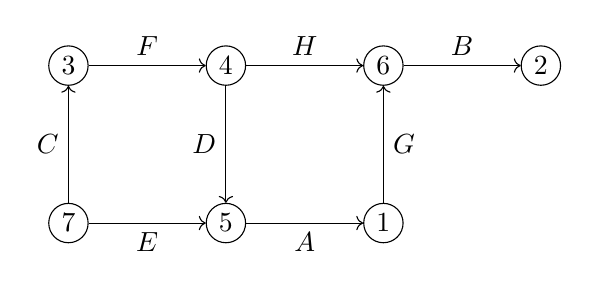
\begin{tikzpicture}[scale = 2,
v/.style={circle, draw, minimum size = 5mm, inner sep = 0pt}]
\node[v] (n7) at (0,0) {$7$};
\node[v] (n3) at (0,1) {$3$};
\node[v] (n5) at (1,0) {$5$};
\node[v] (n4) at (1,1) {$4$};
\node[v] (n1) at (2,0) {$1$};
\node[v] (n6) at (2,1) {$6$};
\node[v] (n2) at (3,1) {$2$};
\draw[->] (n5) to node[auto, swap] {$A$} (n1);
\draw[->] (n6) to node[auto] {$B$} (n2);
\draw[->] (n7) to node[auto] {$C$} (n3);
\draw[->] (n4) to node[auto, swap] {$D$} (n5);
\draw[->] (n7) to node[auto, swap] {$E$} (n5);
\draw[->] (n3) to node[auto] {$F$} (n4);
\draw[->] (n1) to node[auto, swap] {$G$} (n6);
\draw[->] (n4) to node[auto] {$H$} (n6);
\end{tikzpicture}
\end{center}
where the numbers correspond to the rows and the letters to the columns.
\item For this, we again needed a program. The programm you got almost checks every possible determinant, of growing size. The following arguments helped reduce the case spaces a bit, but the algorithm is still exponential, which suffices to find an $7\times 7$ submatrix with determinant not in $\{-1,0,1\}$, but not to find every one of them without spending some good weeks.
\begin{b_item} \item First, such a submatrix should have at least one row from the region involving the identity matrices. Otherwise the determinant would be the product of the determinants of two submatrices of $A$ and thus in $\{-1,0,1\}$.
\item Every row from the region with the identity matrices should hit both diagonals, i.e. have two non-zero entries. Indeed, if all entries are zero, then the matrix has determinant $0$ and if there is only one of them non-zero, the determinant equals $\pm$ the determinant of the matrix without this row and column. We avoided this case, because we were looking for minimal submatrices.
\item There should be at least one column not hitting the diagonal of the respective identity matrix. Indeed, if all columns had a non-zero entry in the region of the identity matrices, then the resulting matrix would look (up to a row-permutation) like:
$$\det\left(\begin{array}{c|c}A'&0\\0&A''\\\hline I_k&I_k\\\end{array}\right)$$
where $k$ is some appropriate integer and both $\left(\begin{array}{c}A'\\0\\\end{array}\right)$ and $\left(\begin{array}{c}0\\A''\\\end{array}\right)$ are some square matrices, where $A',A''$ are submatrices of $A$, on the same column set. The above determinant, due to the fact that $I_k$ permutes with itself equals:
$$\det\left(\begin{array}{c}A'\\-A''\\\end{array}\right)=(-1)^k\det\left(\begin{array}{c}A'\\A''\\\end{array}\right)$$
which is the determinant of a square submatrix of $A$, up to a sign and thus has a value in $-1,0,1$
\end{b_item}
The program first chooses some $\mathrm{num}$ to be the number of rows and columns of the submatrix. Then, it chooses some $\mathrm{kI}\in\left[1,\frac{\mathrm{num}}{2}\right]$ to be the number of choosen rows in the identity-matrices region. Then we choose $\mathrm{kI}$ of $8$ to be these rows, which means that we automatically have chosen $2\mathrm{kI}$ columns as well (we want for these rows to hit both diagonals). Next, we choose $\mathrm{num}-\mathrm{kI}$ rows, among the $14$ rows above, to complete the row choice and $\mathrm{num}-2\mathrm{kI}$ columns, among the ones we did not choose yet to complete the column choice. Then it just checks the determinant.
The first matrix it outputs, for $\mathrm{num}=7$ and $\mathrm{kI}=2$ is the following:
$$\begin{array}{ccccccc}M&=&\begin{array}{c}4\\6\\\phantom{A}\\\phantom{A}\\\phantom{A}\\F\\G\\\end{array}&
\left(\begin{array}{RRR|RRRR}
 1& 0&-1& 0& 0& 0& 0\\
 0& 1& 1& 0& 0& 0& 0\\\hline
 0& 0& 0& 1& 0& 0&-1\\
 0& 0& 0& 0&-1& 1& 0\\
 0& 0& 0&-1& 1& 0& 0\\\hline
 1& 0& 0& 0& 0& 1& 0\\
 0& 1& 0& 0& 0& 0& 1\\
\end{array}\right)&
\begin{array}{c}\phantom{A}\\\phantom{A}\\1\\4\\5\\\phantom{A}\\\phantom{A}\\\end{array}\\
\\
&&&\begin{array}{RRR|RRRR}
F&G&H&A&D&F&G\\
\end{array}\\
\end{array}$$
with \href{https://www.wolframalpha.com/input/?i=det\%5B(1,0,-1,0,0,0,0),(0,1,1,0,0,0,0),(0,0,0,1,0,0,-1),(0,0,0,0,-1,1,0),(0,0,0,-1,1,0,0),(1,0,0,0,0,1,0),(0,1,0,0,0,0,1)\%5D}{$\det(M)=2$}. The numbers and the letters refer to the rows and columns of the original matrix $A$.
\item Due to the Thm of Hoffman and Kruskal (1956) totally unimodular matrices $A$ are characterized by the fact that the extreme points of $\{x|Ax\leq b\}$ are integer, for any integer $b$. This means, that for the $22\times 16$ matrix $B$ of (b) there exists some $c\in\mathbb{Z}^{16}$ and $b\in\mathbb{Z}^{22}$ such that:
$$\mathrm{arg}\max_{x\in\mathbb{R}^{22}}\{c^Tx:Bx\leq b\}\not\subseteq\mathbb{Z}^{16}$$
or at least, it should in theory. Let:
$$A=\left(\begin{array}{ccccccc}
1&-1&-1&0&0&0&0\\
0&1&0&-1&-1&0&0\\
0&0&1&1&0&-1&0\\
0&0&0&0&1&1&-1\\
\end{array}\right)$$
This matrix is the incident matrix of the following directed graph, having removed the rows corresponding to vertices $s,t$:
\begin{center}
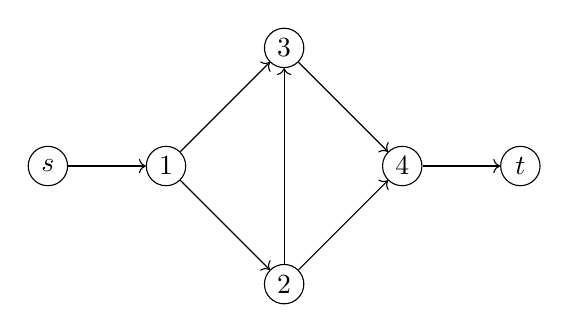
\begin{tikzpicture}[scale = 1.5,
v/.style={circle, draw, minimum size = 5mm, inner sep = 0pt}]
\node[v] (s) at (-2,0) {$s$};
\node[v] (1) at (-1,0) {$1$};
\node[v] (2) at (0,-1) {$2$};
\node[v] (3) at (0,1) {$3$};
\node[v] (4) at (1,0) {$4$};
\node[v] (t) at (2,0) {$t$};
\draw[->] (s) to (1);
\draw[->] (1) to (2);
\draw[->] (1) to (3);
\draw[->] (2) to (3);
\draw[->] (2) to (4);
\draw[->] (3) to (4);
\draw[->] (4) to (t);
\end{tikzpicture}
\end{center}
It is easy to see that $A$ is TU and that the construction of (b) for $A$ is TU iff the construction of (b) for $A'$ is TU, where $A'$ is $A$ without the first and the last column. The program {\rm 2c.cpp} proves that the matrix
$$B'=\left(\begin{array}{cc}A'&0\\0&A'\\I&I\\\end{array}\right)$$
is not totally unimodular. The code in {\rm 2c.sh} tries to solve a general max 2-commodity flow in the above graph, with common source $s$ and common target $t$, with positive integer (and random) cost, balance, capacity, many times in a row but unfortunately fails to find one with non-integer solution, even though the matrix $B$ of the constraints is exactly:
$$B=\left(\begin{array}{cc}A&0\\0&A\\I&I\\\end{array}\right)$$
and thus not TU.
\end{a_enum}
\end{document}
